
\section{Ejercicio 6}

\subsection{Introducción}

En este ejercicio se realizará el diseño de un circuito que adapta una señal de tensión proveniente de un sensor de temperatura LM324. 
Luego, se implementará el mismo en un PCB y se analizarán los resultados obtenidos.

\subsection{Diseño del circuito}

Como primer paso se deben definir las entradas y salidas del sistema para poder comenzar con su diseño. Respecto a la entrada, la fuente de la misma es el sensor de temperatura LM324.
 Según se pudo consultar en su datasheet, la ganancia del mismo es de $100 \frac{mV}{°C}$.Por otro lado, el rango de temperaturas especificado de funcionamiento del circuito va desde $35°C$ hasta $45°C$.
 Luego, el rango de tensiones de entrada es de $350mV$ a $450mV$, lineal respecto de la temperatura. El rango de salida del circuito está comprendido entre $0V$ y $5V$, a  $35°C$ y $45°C$ respectivamente. 

 
 Como se puede observar, tanto la entrada como la salida del circuito son rangos lineales, por lo que la adaptación implica solamemte un escalamiento y un corrimiento aplicados sobre la señal de entrada.
  Teniendo en cuenta los circuitos típicos observados en clase se decidió emplear un sumador inversor conectado en cascada a un amplificador inversor, como se puede observar en la figura~\ref{fig:EJ6_circuito}.  
  
\begin{figure}[H]
    \centering
    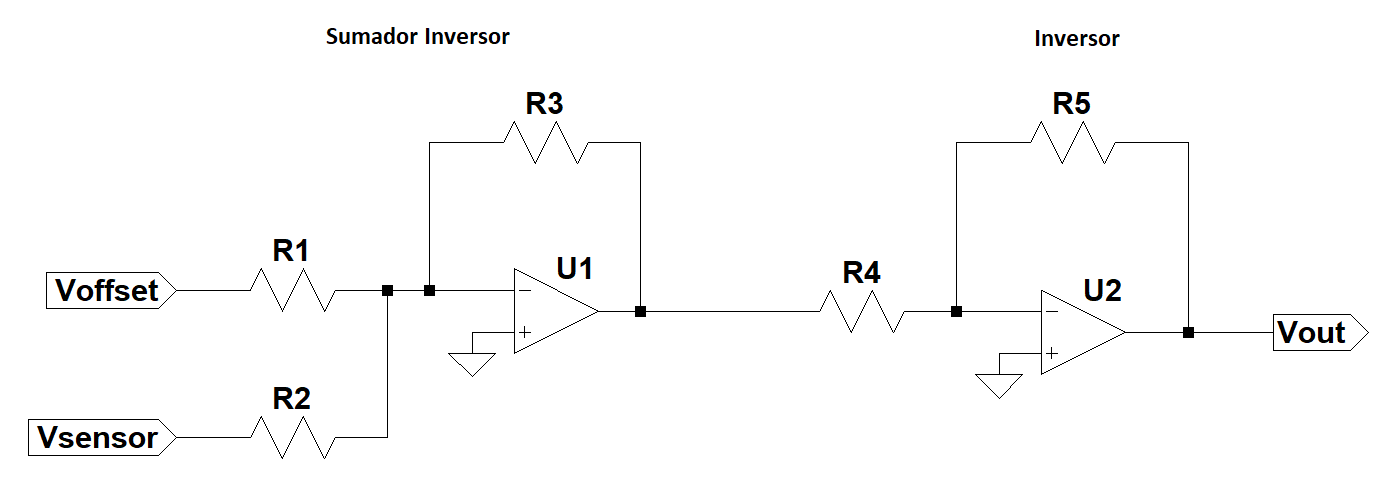
\includegraphics[width=0.9\textwidth]{../EJ_6/Captures/EJ6_circuito_teorico.png}
    \caption{Circuito adaptador}
    \label{fig:EJ6_circuito} 
\end{figure}

Dado que se utilizan dos amplificadores operacionales se creyó conveniente emplear el integrado TL082. La ecuación que caracteriza a dicho circuito se reproduce a continuación.

\begin{equation}
    v_{out}= \left( - \frac{R_3}{R_2} \cdot v_{sensor}  - \frac{R_3}{R_1} \cdot v_{offset} \right) \cdot \left( -\frac{R_5}{R_4}   \right)
    \label{fig:EJ6_ecuacion_sistema} 
\end{equation}

Si suponemos que el amplificador inversor tiene ganancia unitaria (esto es, $R_5=R_4$), y que la tensión que se usará como offset es $-V_{cc}$ obtenemos

\begin{equation}
    v_{out}= \frac{R_3}{R_2} \cdot v_{sensor}  - \frac{R_3}{R_1} \cdot v_{cc} 
    \label{fig:EJ6_ecuacion_sistema2} 
\end{equation}

En la ecuación anterior se pueden apreciar las dos etapas de adaptación mencionadas anteriormente (escalamiento y corrimiento). Ahora si operamos sobre esta simplificación obtenemos

\begin{equation}
    \frac{R_3}{R_2} \cdot \left( v_{sensor} - \frac{R_2}{R_1} \cdot v_{cc} \right)
    \label{fig:EJ6_ecuacion_sistema_simplificada_final} 
\end{equation}

Si decidimos fijar $R_2$ entonces agregando presets en serie a $R_1$ y $R_3$ podremos ajustar de forma independiente el corrimiento y escalamiento, respectivamente.
Realizando los c\'alculos apropiados para conocer los valores de los resistores se llega a la siguiente expresi\'on:

\begin{equation}
    Aca van las equivalencias entre resistores
    \label{fig:EJ6_ecuacion_resistores}
\end{equation}

Con las equivalencias anteriores y fijando un valor comercial para el resistor $R_2$ se pueden calcular los valores teóricos de resistencia para $R_1$ y $R_3$.
  Luego se normalizan estos valores, al valor comercial inmediato inferior que tambi\'en se encuentre disponible en el pa\~nol de la facultad.
  Por \'ultimo se agregan dos presets de $100k\Omega$ en serie a $R_1$ y $R_3$ para poder efectuar la calibraci\'on del circuito. Se obtiene la configuraci\'on que se detalla en la tabla de abajo.


